\section{Phase II Step 2: C2 Interpretability Analysis}
\label{sec:phase2_c2_interpretability}

The second Month 3 criterion evaluates whether each candidate metric can be explained clearly and audited
without relying on hidden assumptions. This step is deliberately separated from C1 stability: a metric can be
stable but weak as a reputation signal, or meaningful but harder to explain. The C2 evidence therefore scores
interpretability, not final suitability.

\subsection{Scoring protocol and artifacts}
\label{sec:c2_protocol_artifacts}

C2 uses a fixed five-dimension rubric. Each dimension is scored on a 0--2 scale:
\textbf{0} means weak, \textbf{1} means partial, and \textbf{2} means clear. The maximum score is 10.
The rubric is generated as a CSV artifact so that the score basis remains explicit.

\begin{table}[H]
\centering
\scriptsize
\renewcommand{\arraystretch}{1.08}
\begin{tabularx}{\textwidth}{p{2.1cm}p{3.6cm}X}
\toprule
\textbf{Dimension} & \textbf{Name} & \textbf{Meaning} \\
\midrule
C2\_D1 & Semantic clarity & Whether the metric has a plain and stable meaning. \\
C2\_D2 & Unit clarity & Whether the unit can be explained without ambiguity. \\
C2\_D3 & Normalization clarity & Whether normalization improves comparison without obscuring meaning. \\
C2\_D4 & Tooling transparency & Whether extraction can be reproduced from explicit inputs. \\
C2\_D5 & Reputation explanation fit & Whether the metric can support a developer-reputation explanation. \\
\bottomrule
\end{tabularx}
\caption{C2 interpretability rubric. Each dimension is scored from 0 to 2.}
\label{tab:c2_rubric}
\end{table}

\begin{table}[H]
\centering
\scriptsize
\renewcommand{\arraystretch}{1.08}
\begin{tabularx}{\textwidth}{p{5.0cm}rX}
\toprule
\textbf{Artifact} & \textbf{Rows} & \textbf{Role} \\
\midrule
\path{out/c2_interpretability_rubric_all.csv} & 5 & Fixed C2 scoring dimensions and definitions. \\
\path{out/c2_interpretability_scores_all.csv} & 25 & Per-metric, per-dimension scores with written rationales. \\
\path{out/c2_interpretability_summary_all.csv} & 5 & Metric-level total score, band, strongest dimensions, and weakest dimensions. \\
\path{logs/c2_interpretability_20260508.log} & 1 & Execution log for the C2 scoring run. \\
\bottomrule
\end{tabularx}
\caption{Phase II C2 interpretability artifacts. Paths are relative to the Phase II analysis directory.}
\label{tab:c2_artifacts}
\end{table}

\subsection{C2 results}
\label{sec:c2_results}

\begin{table}[H]
\centering
\scriptsize
\renewcommand{\arraystretch}{1.08}
\begin{tabularx}{\textwidth}{p{0.8cm}p{3.2cm}p{2.0cm}ccX}
\toprule
\textbf{ID} & \textbf{Metric} & \textbf{Status} & \textbf{Score} & \textbf{Band} & \textbf{Interpretation} \\
\midrule
M3 & Activity cadence & Implemented & 9/10 & High & Clearest activity-continuity signal; still should not be treated as quality by itself. \\
M1 & Snapshot size & Implemented & 8/10 & High & Very easy to explain and reproduce, but mainly useful as context rather than reputation evidence. \\
M2 & Churn & Implemented & 8/10 & High & Easy to explain as change magnitude, with normalization and quality caveats. \\
M4 & Ownership/concentration & Implemented & 7/10 & Medium & Strong reputation relevance, but shares, Gini, and identity aggregation require careful explanation. \\
M5 & Maintenance responsiveness & Design extension & 6/10 & Medium & Conceptually useful, but excluded from the current empirical decision because issue/PR event data were not collected. \\
\bottomrule
\end{tabularx}
\caption{C2 interpretability summary for the candidate metrics.}
\label{tab:c2_interpretability_summary}
\end{table}

\begin{figure}[H]
\centering
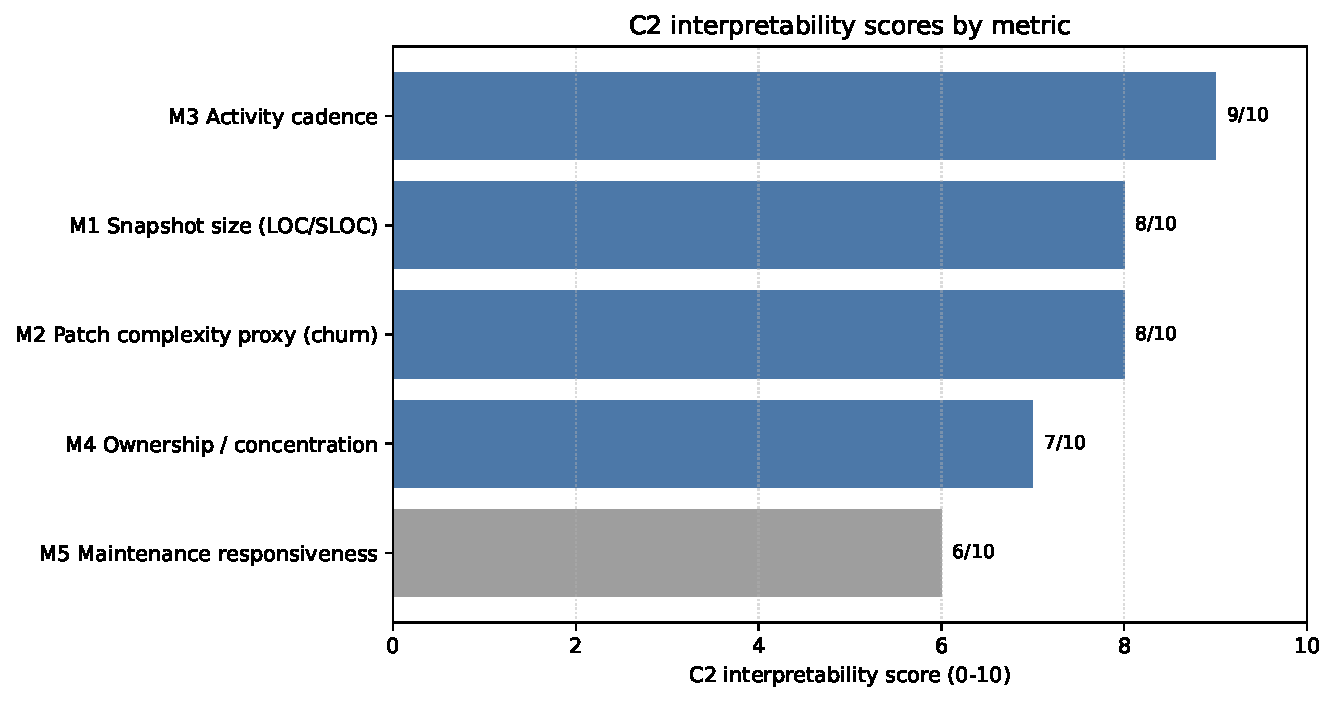
\includegraphics[width=0.90\textwidth]{figures/month3_c2/c2_interpretability_scores.pdf}
\caption{C2 interpretability scores on a 0--10 scale. The design-extension metric is shown separately from implemented metrics.}
\label{fig:c2_interpretability_scores}
\end{figure}

The C2 result strengthens the distinction between simple measurement and useful reputation evidence. M3 receives
the highest interpretability score because commits, active days, and commits/day are easy to explain and the
duration normalization is direct. However, the interpretation remains bounded: activity continuity is not the
same as contribution quality. M1 and M2 also score highly because their units are transparent. Their weakness is
not readability but meaning: M1 describes project size, and M2 describes change magnitude rather than quality.

M4 receives a lower interpretability score, but it remains important. Ownership and concentration are closer to
maintainer responsibility, yet they require more explanation because Gini, top-contributor shares, and identity
canonicalization are less immediate than counts or rates. M5 remains a design extension. Its concept is clear,
but the current evidence base intentionally excludes issue and pull-request event data, so it should not compete
with the implemented candidates in the current empirical decision.

\subsection{C2 interpretation for the decision process}
\label{sec:c2_interpretation}

C2 does not eliminate any implemented metric. Instead, it defines how each candidate should be discussed in the
remaining comparison:
\begin{itemize}[leftmargin=*]
  \item M1 can support context and normalization claims, but not direct developer-reputation claims.
  \item M2 can support effort and change-magnitude claims, but it needs safeguards against reading churn as quality.
  \item M3 is the easiest implemented reputation-adjacent signal to explain, especially after duration normalization.
  \item M4 has the strongest conceptual link to maintainer influence, but it must be presented with clear definitions and identity rules.
  \item M5 should remain documented for future work and should not be selected for the baseline PoC unless new event data are added.
\end{itemize}

The next criterion is C3 gaming resistance. That step should focus on how easily each metric can be manipulated
and whether manipulation can be detected from the existing Phase I evidence.
